\section{Dynamisches Verhalten}

\subsection{Login/Registrierung}
%TODO Image here
\subsection{Aktivität erledigen}

\begin{figure}[H]
  \centering
  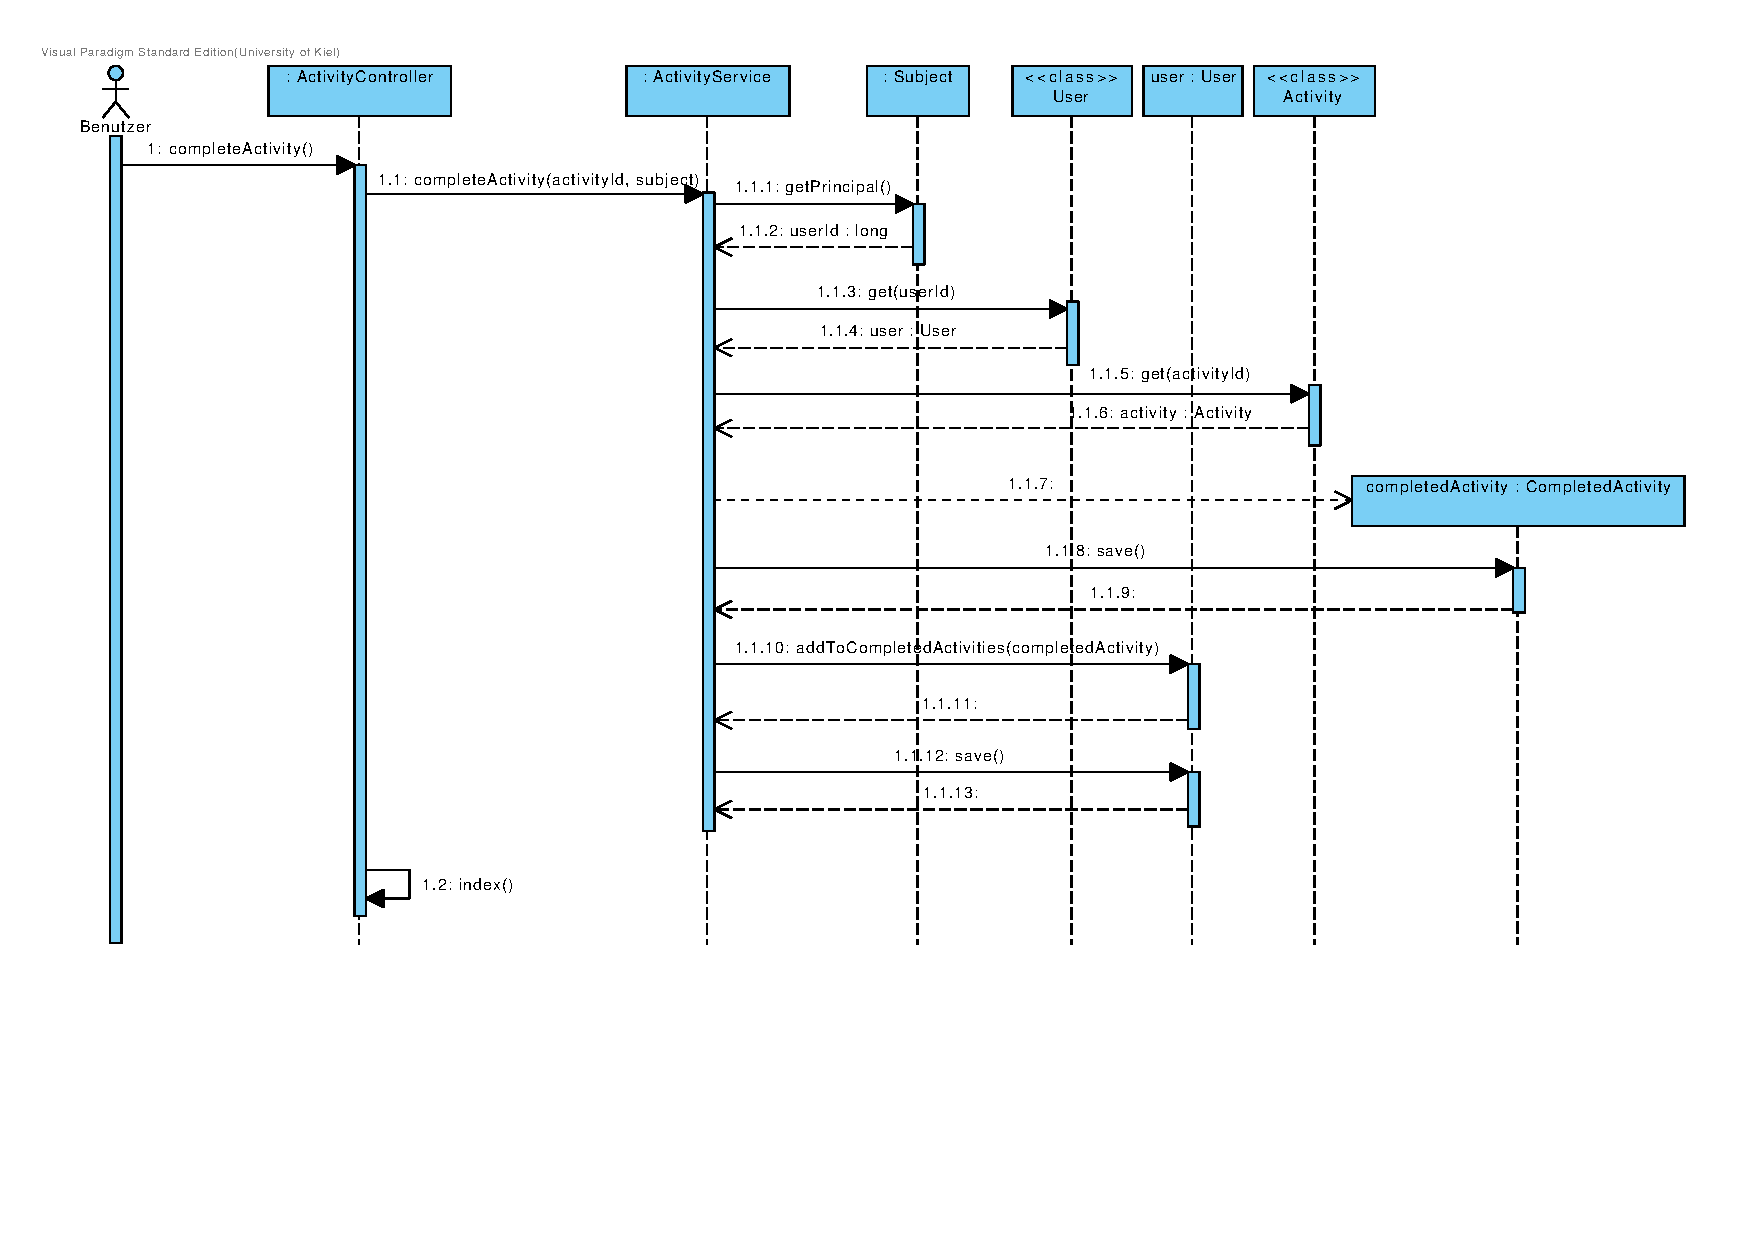
\includegraphics[width=\textwidth, clip]{gfx/aktivitaet_erledigen}
  \caption{Eine Aktivität erledigen}
\end{figure}

Der eingeloggte Benutzer gelangt über einen Klick auf „Aktivitäten“
auf die Aktivitätenseite. Auf dieser findet er die Liste mit
Aktivitäten. Durch das Klicken auf die zu erledigende Aktivität werden
dem Benutzer die entsprechenden Punkte gutgeschrieben und die
erledigte Aktivität wird für den Benutzer gesperrt bis die festgelegte
Sperrphase abgelaufen ist. Der Benutzer wird dadurch außerdem wieder auf die
Aktivitätenseite zurück geleitet.

Alternativ ist das Erledigen favorisierter Aktivtäten auch auf der
Landingpage möglich.

\subsection{Rangliste ansehen}
%TODO Image here
Der eingeloggte Admin kann ein Team über einen speziellen Button, welcher die Funktion blockTeam(teamId) aufruft, sperren. Dabei wird das Team und nacheinander jedes einzelne Teammitglied gesperrt. Nachdem dies geschehen ist, tauchen auch das Team und deren Mitglieder nicht mehr in der Teilnehmerliste auf.\\

\subsection{Team erstellen}
\begin{figure}[H]
  \centering
  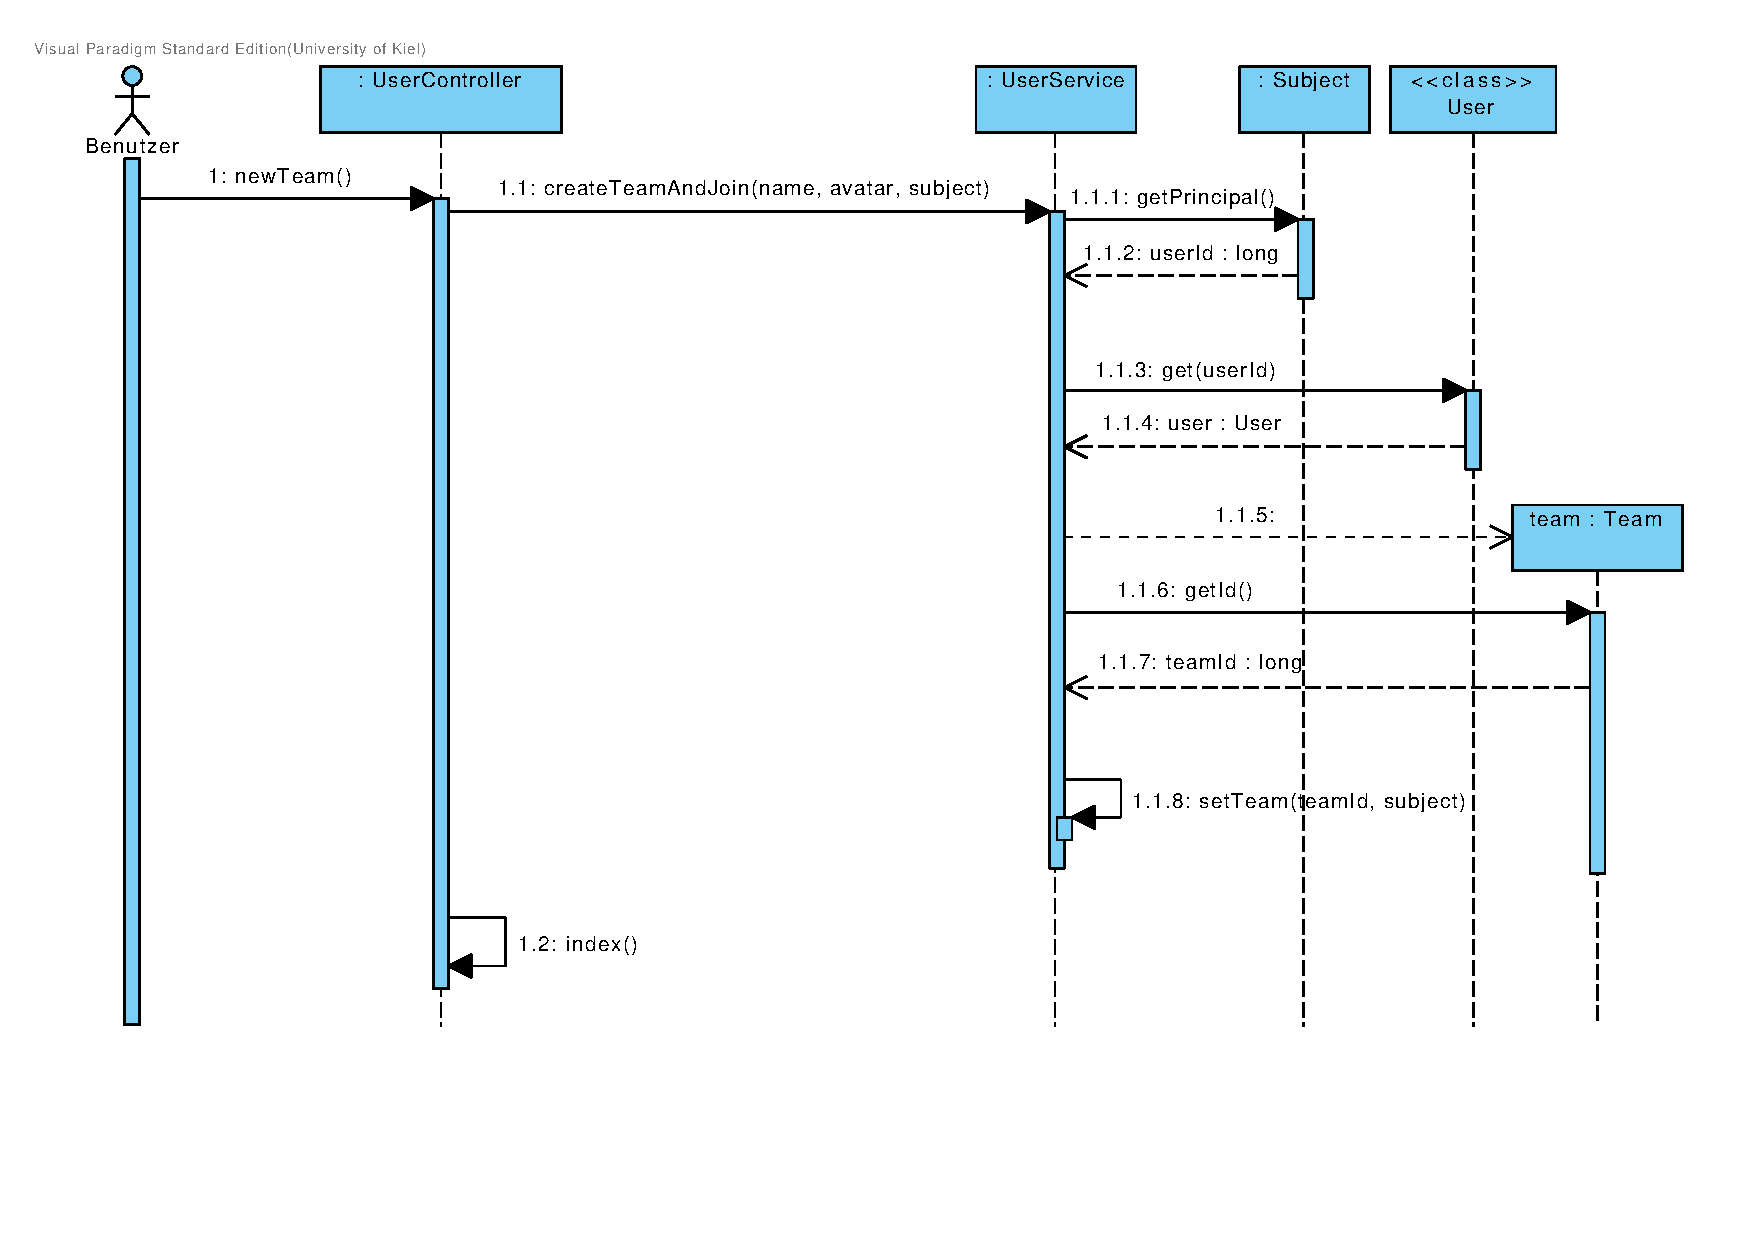
\includegraphics[width=\textwidth, clip]{gfx/team_erstellen}
  \caption{Ein Team erstellen}
\end{figure}

Der eingeloggte Benutzer, welcher noch kein Mitglied eines Teams ist,
kann auf seiner Landingpage über den Link „Team erstellen“ ein neues
Team generieren. Der Benutzer gelangt auf eine leere Teamprofilseite,
in der er den Teamnamen, ein Teamfoto und eine Beschreibung des Teams
eingeben kann. Anschließend bestätigt der Benutzer über einen Klick
auf „Team gründen“ sein Team. Mit der Bestätigung ist der Benutzer
automatisch dem Team beigetreten. Die Teamprofilseite aktualisiert
sich und der Benutzer sieht seine neue Teamprofilseite mit ihm als
Mitglied.\\

\subsection{Team blocken}
%TODO Image here
Der eingeloggte Admin kann ein Team über einen speziellen Button, welcher die Funktion blockTeam(teamId) aufruft, sperren. Dabei wird das Team und nacheinander jedes einzelne Teammitglied gesperrt. Nachdem dies geschehen ist, tauchen auch das Team und deren Mitglieder nicht mehr in der Teilnehmerliste auf.\\

\subsection{Vorschlag erstellen}
\begin{figure}[H]
  \centering
  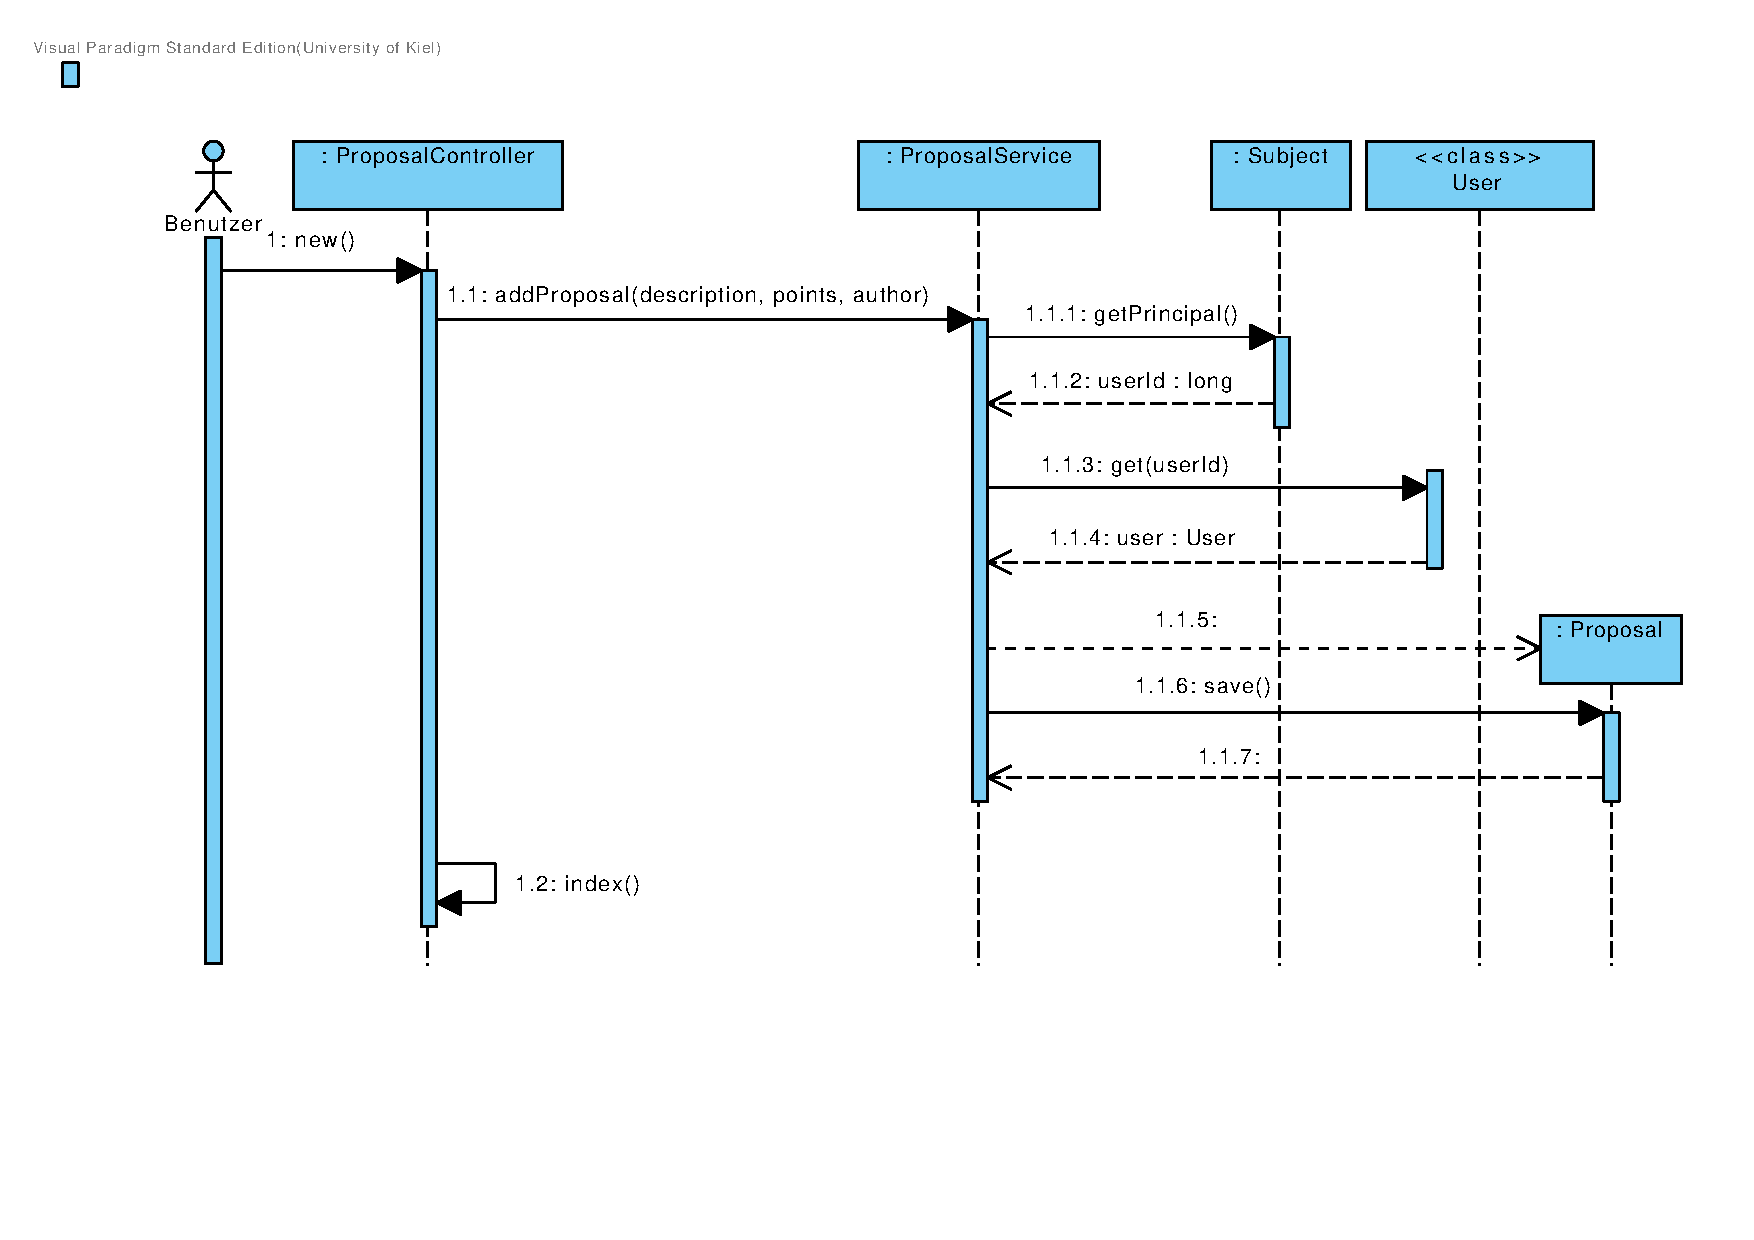
\includegraphics[width=\textwidth, clip]{gfx/vorschlag_erstellen}
  \caption{Einen Vorschlag erstellen}
\end{figure}

Der eingeloggte Benutzer, kann auf der Vorschlagsseite über den Link
``eine neue Aktivität vorschlagen'' einen neuen Vorschlag für eine
Aktivität einreichen. Der Benutzer gelangt über den Link auf eine
Seite, auf welcher er eine Beschreibung und eine Punktzahl für seinen Vorschlag
 eingeben kann. Auf dieser Seite kann der Benutzer durch Klick auf
 ``Vorschlag einreichen'' den Vorschlag einreichen. Anschließend sieht
 der Benutzer die Bestätigung ``Vorschlag erfolgreich eingereicht''
 und wird auf die Vorschlagsseite zurückgeleitet, wo er seinen
 Vorschlag einesehen kann.
 
\subsection{Vorschlag bewerten}
\begin{figure}[H]
  \centering
  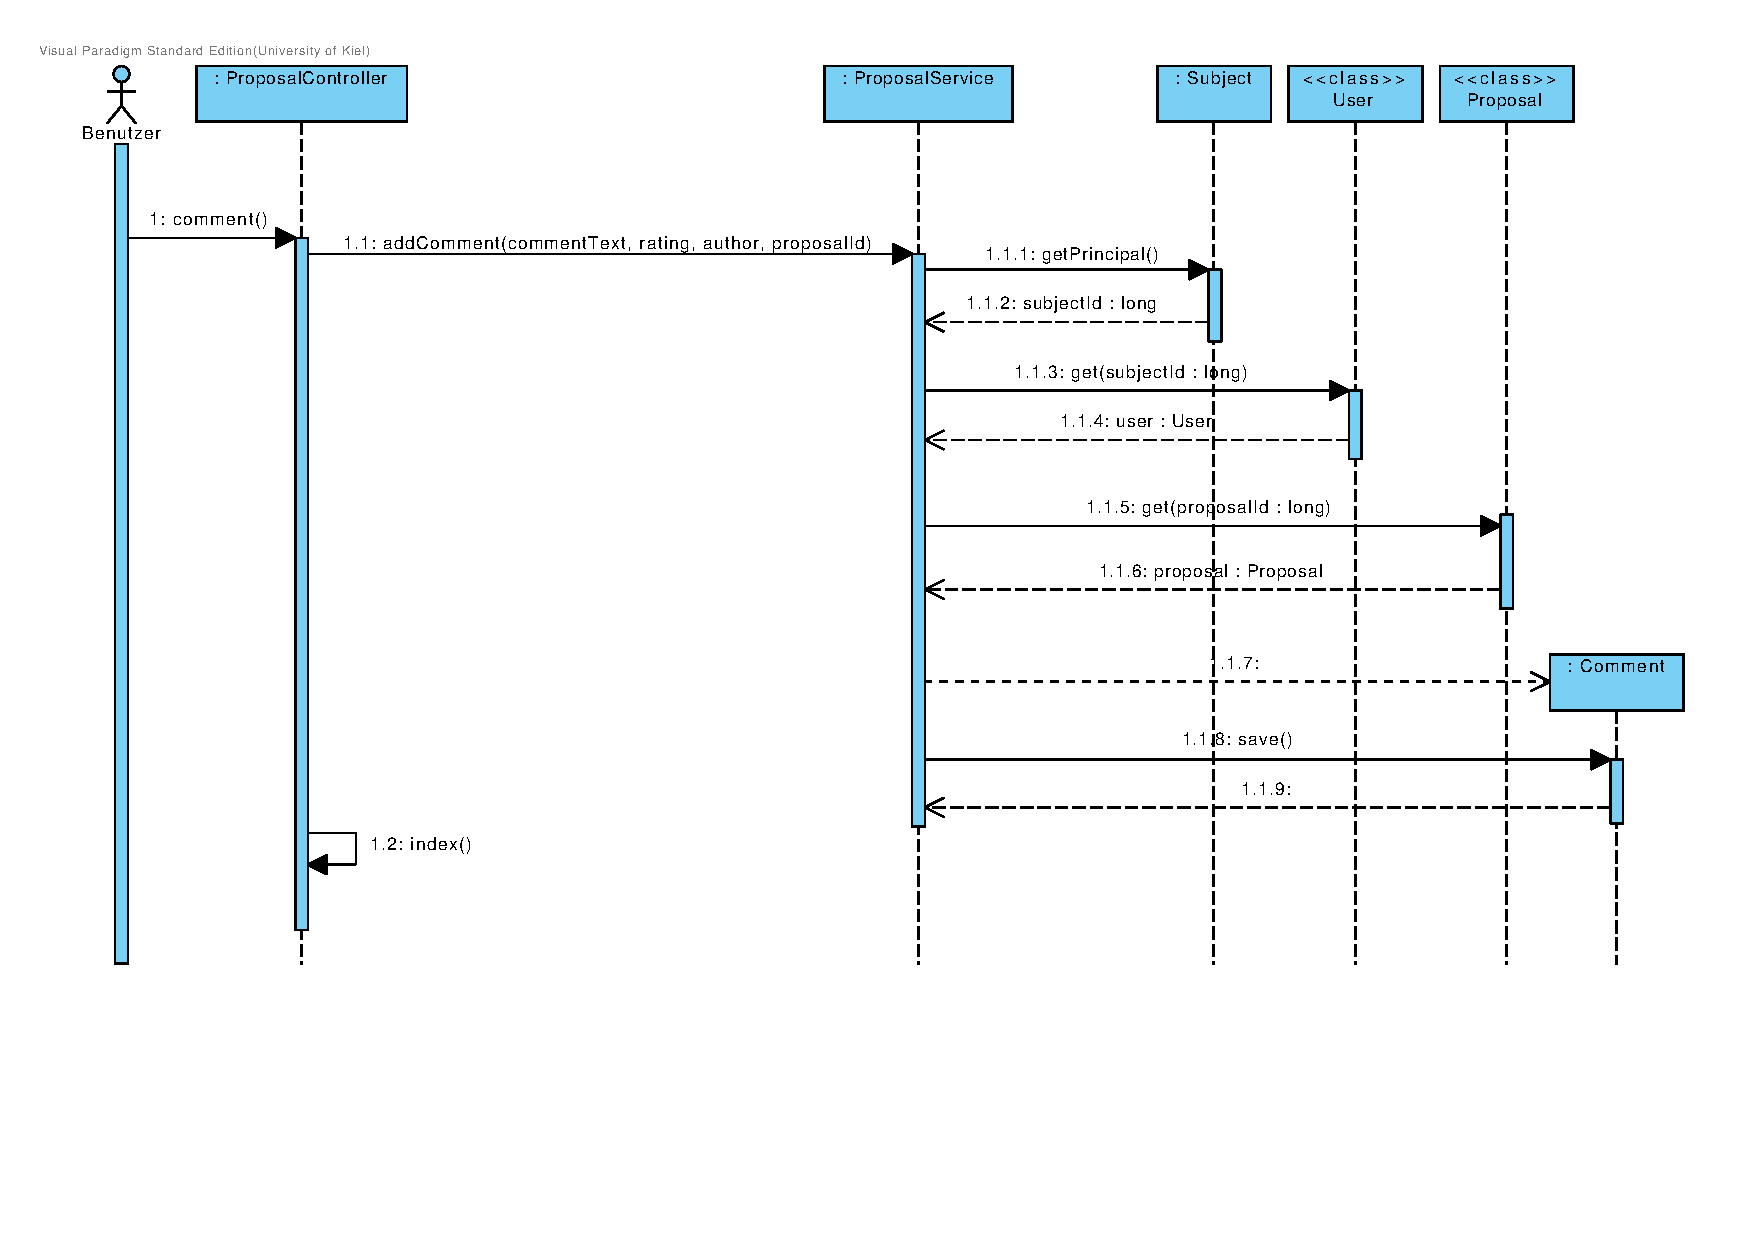
\includegraphics[width=\textwidth, clip]{gfx/vorschlag_bewerten}
  \caption{Einen Vorschlag bewerten}
\end{figure}

Der eingeloggte Benutzer, kann auf der Vorschlagsseite über den Link
``diesen Vorschlag bewerten'', welcher bei jedem Vorschlag angezeigt
wird, eine Bewertung zu jedem eingereichten Vorschlag abgeben. Durch
Klick auf diesen Link gelangt der Benutzer auf eine Seite, auf welcher
er ein Kommentar und/oder eine Bewertung in Form von 1 bis 5 Sternen
abgeben kann. Auf dieser Seite kann der Benutzer durch Klick auf
 ``Bewertung abgeben'' die Bewertung abgeben. Anschließend sieht
 der Benutzer die Bestätigung ``Bewertung abgegeben'' und wird auf die Vorschlagsseite zurückgeleitet.
 

\subsection{Statistiken exportieren}
%TODO Image here
Der eingeloggte Benutzer klickt auf Statistik und gelangt auf die Statistikseite, wo er auf den Button „Herunterladen“ klickt. Nun wird dem Benutzer ein Download zur Verfügung gestellt, welcher ihm ermöglicht, die Statistiken in einer „.csv“-Datei auf dem eigenen Computer zu speichern.\\
\subsection{Vorschlag in Aktivität umwandeln}
%TODO Image here
\subsection{App: Benutzerrangliste ansehen}
Die Serveranfragen in der App funktionieren alle nach dem selben Muster. Benutzerrangliste ansehen steht hier exemplarisch für weitere Anwendungsfälle dieser Art.
%TODO Image here
Wenn der Nutzer in der App zur Benutzerrangliste navigiert, wird diese automatisch bei der Erstellung des \emph{Fragments} geladen. Dabei wird auf ein \emph{GetUserRankingTask} die Methode \emph{execute()} aufgerufen. \emph{GetUserRankingTask} erbt von \emph{AccessServerTask}, die wiederum von der Androidklassse \emph{AsyncTask} erbt. In dem \emph{AccessServerTask} wird die Methode \emph{doInBackground()} aufgerufen, die wiederum die Methode \emph{createServerRequest} aufruft, die im \emph{GetUserRankingTask} definiert ist.\\
Sobald die \emph{doInBackground()}-Methode fertig ausgeführt wurde, wird (vom \emph{AsyncTask}) die Methode \emph{onPostExecute()} aufgerufen, die \emph{handleServerResponse()} des \emph{GetUserRankingTask} ausführt. Hier wird dann die Darstellung im \emph{Fragment} getätigt.\\
Der Vorteil dieser Art der Implementierung ist, dass nur einmal eine generelle Serverabfrage definiert werden muss, und sich keine weitere Gedanken um dessen Implementierung gemacht werden m\"ussen. Deswegen ist die Durchführung der HTTP-Abfrage hier auch nicht weiter aufgeführt.